%\documentstyle[epsf,twocolumn]{jarticle}       %LaTeX2e仕様
\documentclass[twocolumn]{jarticle}     %pLaTeX2e仕様(platex.exeの場合)
% \documentclass[onecolumn]{ujarticle}   %pLaTeX2e仕様(uplatex.exeの場合)
%%%%%%%%%%%%%%%%%%%%%%%%%%%%%%%%%%%%%%%%%%%%%%%%%%%%%%%%%%%%%%
%%
%%  基本バージョン
%%
%%%%%%%%%%%%%%%%%%%%%%%%%%%%%%%%%%%%%%%%%%%%%%%%%%%%%%%%%%%%%%%%
\setlength{\topmargin}{-45pt}
%\setlength{\oddsidemargin}{0cm}
\setlength{\oddsidemargin}{-7.5mm}
%\setlength{\evensidemargin}{0cm}
\setlength{\textheight}{24.1cm}
%setlength{\textheight}{25cm}
\setlength{\textwidth}{17.4cm}
%\setlength{\textwidth}{172mm}
\setlength{\columnsep}{11mm}

%\kanjiskip=.07zw plus.5pt minus.5pt


% 【節が変わるごとに (1.1)(1.2) … (2.1)(2.2) と数式番号をつけるとき】
%\makeatletter
%\renewcommand{\theequation}{%
%\thesection.\arabic{equation}} %\@addtoreset{equation}{section}
%\makeatother

%\renewcommand{\arraystretch}{0.95} 行間の設定
%%%%%%%%%%%%%%%%%%%%%%%%%%%%%%%%%%%%%%%%%%%%%%%%%%%%%%%%
%\usepackage{graphicx}   %pLaTeX2e仕様(\documentstyle ->\documentclass)
\usepackage[dvipdfmx]{graphicx}
\usepackage{subcaption}
\usepackage{multirow}
\usepackage{amsmath}
\usepackage{url}
\usepackage{ulem}
\usepackage{algorithm}
\usepackage{algorithmic}
\usepackage{listings} %,jlisting} %日本語のコメントアウトをする場合jlistingが必要
%ここからソースコードの表示に関する設定
\lstset{
  basicstyle={\ttfamily},
  identifierstyle={\small},
  commentstyle={\smallitshape},
  keywordstyle={\small\bfseries},
  ndkeywordstyle={\small},
  stringstyle={\small\ttfamily},
  frame={tb},
  breaklines=true,
  columns=[l]{fullflexible},
  numbers=left,
  xrightmargin=0zw,
  xleftmargin=3zw,
  numberstyle={\scriptsize},
  stepnumber=1,
  numbersep=1zw,
  lineskip=-0.5ex
}
%%%%%%%%%%%%%%%%%%%%%%%%%%%%%%%%%%%%%%%%%%%%%%%%%%%%%%%%
\begin{document}

	%bibtex用の設定
	%\bibliographystyle{ujarticle}

	\twocolumn[
		\noindent
		\hspace{1em}
		前期研究発表会資料 2022 年 7 月 6 日 (水)
		\hfill
	  M2 杉山 竜弥
		\vspace{2mm}

		\hrule
		\begin{center}
			{\Large \bf 手描きスケッチの類似度}
		\end{center}
		\hrule
		\vspace{9mm}
	]

\section{はじめに}

% 予定
% tho report    実験・まとめ
% wed           実験・ぱわぽ
% thu yasumu    ぱわぽ
% fri deadline  このよのおわり
%
% sat
% sun
%
% mon
% tho
% wed

  近年,機械学習の発展を背景に人工知能 (Artificial Intelligence : AI) が注目を浴びている.
  AI は単純なパターン認識では人間の能力を凌駕する性能を示す一方で,人間の情緒や感性に関する分野,特に人間の創作物への AI の適用はいまだ困難である.
  創作物の中でも,スケッチは,年齢,国籍,文化にかかわらず,幅広く共感可能な表現であるため重要度が高い.
  このため,感性を取り扱う分野での重要な AI の課題の 1 つとされてきた.\par

  著者らはこれまで計算機と人間とのコミュニケーションを実現するため,Creative Animating Sketchbook (CASOOK) を提案してきた.
  従来の研究において,CASOOK は描き順の情報を持たない静止画像のみを対象としていたが,CASOOK の拡張として描き順を扱うために,深層学習モデルである sketch-rnn \cite{DBLP:journals/corr/HaE17} を導入した Creative Animating Sketchbook with sketch-rnn (CASOOK-SR) を提案している.
  この手法では,描き順の決定プロセスが潜在意識下にあるという観点から,画像と同程度に人間の感性が描き順に含まれていることに着目している.
  しかしながら,生成された手描きスケッチを定量的に評価するために必要な類似性の比較は困難な課題の 1 つであった.
  この課題の解決のため,本稿ではペンの動きだけでなく形も評価に取り入れた,手描きスケッチの類似性に関する客観的な評価モデルを定義し,その有効性を実験によって確認する.


\section{要素技術}

  \subsection{Sketch-rnn}	\label{tau}
    sketch-rnn とは深層学習を用いて,人間がイラストを描くときの一連の描き順を学習することでユーザのイラストを補完,推測する深層学習を利用したモデルである.
    % 図 \ref{fig:one} に sketch-rnn の学習モデルを構成する Variational Autoencoder (VAE) \cite{NIPS2017_7011} を示す.
    sketch-rnn の学習モデルは Variational Autoencoder (VAE) を基に構成されている.
    入力はスケッチの時系列を含む描き順を意味する行列であり,潜在ベクトルがエンコーダの出力となる.
    また,デコーダの出力は入力と同じ,画像を生成できる行列となる.


	\subsection{描き順データ}
		Google が公開する描き順データセットである QuickDraw! \cite{Cheema:2012:QID:2207676.2208550} の形式を使用する.
		この形式では, 1 つの手描きスケッチを構成する描き順データは行列で保持される.
		描き順データの行方向は手描きスケッチの描き始めから描き終わりまでのペンの状態に関する情報を時系列に沿って保持する.
		また,描き順データの列方向はある時刻 $t$ におけるペンの状態を保持しており,$x$ 座標の相対値, $y$ 座標の相対値,ストロークの描き終わりのブール値をそれぞれベクトルで持っている.

    \subsection{cos類似度}
コサイン類似度は、そのまま、ベクトル同士の成す角度の近さを表現するため、三角関数の普通のコサインの通り、1に近ければ類似しており、0に近ければ似ていないことになる。

\begin{equation}
  \cos( \overrightarrow{a}, \overrightarrow{b} ) =
  \frac{\overrightarrow{a} \cdot \overrightarrow{b}}{|\overrightarrow{a}| |\overrightarrow{b}|}
\end{equation}

    \subsection{akaze}
類似画像検索は任意の画像に対して類似している画像
を探すことである. 本研究では, 類似画像検索のアルゴ
リズムとして Accelerated KAZE (AKAZE) \cite{alcantarilla2011fast} とヒス
トグラム比較を用いた. AKAZE は特徴点およびその特
徴量を抽出するアルゴリズムの一つであり, 拡大縮小や
回転に強いという利点がある. 本研究における類似度の
計算には特徴点マッチングをし, 距離の平均を取るとい
う手法を用いた. 特徴点マッチングでは距離を算出して
いるため同一画像の場合, 類似度は 0 となり, 値が小さ
くなるほど類似度が高いことを示す. ヒストグラムは横
軸を画素値, 縦軸を画素値の出現頻度と設定したグラフ
である. ヒストグラムから画像のコントラスト, 明るさ,
画素値の分布を確認することができる. ヒストグラム比
較では主に色を用いた類似画像検索が可能となっている.
% 本研究では AKAZE, ヒストグラム比較のそれぞれにお
% いて類似度が高い上位 5 枚の画像の中で, AKAZE, ヒス
% トグラム比較の両方に含まれている画像が任意の画像に
% 対する類似画像と設定した. 本実験では類似画像検索を
% GAN の生成画像に対して用いることで, 生成画像が単に
% GAN の訓練データと類似している画像となっていない
% かの裏付けとして用いた.

\section{提案手法}

絵描き歌自動生成システムの成果についてまとめる.
\begin{itemize}
  \item スケッチの類似性を評価する指標を提案.
  \item 手描きスケッチをストローク(1筆)に分解して,類似するデータラベルから絵描き歌のベースとなる指示を作成.
\end{itemize}
課題については,文章が英語であることなどが挙げられていた.

絵描き歌の生成という機能を 2 段階に分けると,スケッチから歌詞への変換と,歌詞から曲への変換に分けられる.
したがって事前調査として,「画像から文章への変換」や「作曲の自動化」などについて調べた.

\subsection{画像から文章への変換}
先行研究では,スケッチから推測した単語列をもとに絵描き指示を生成していた.

他の方法では,
スケッチではないが画像からキャプションを生成する研究(\cite{vinyals2015show}など)がある.
この方針の場合,英語ではなく日本語で絵描き歌用のデータセットを作成する必要があるため,先行研究の方法よりも難しいと思われる.

\subsection{作曲の自動化}
機械学習による作曲も,入力と出力によって問題の種類が様々あった.
メロディー以外にも音楽の要素は多数存在し,
生成方法も小節単位や時間単位,音符単位などがあり,
データフォーマットも 音声信号,MIDI,ピアノロール,テキスト形式があった.

音楽に関する知識がないので,「作曲の自動化」についてはかなり厳しいと感じた.

% \section{方針}
「作曲の自動化」はかなり難しいと分かったため,「画像から文章への変換」に絞る方針にしたい.

先行研究で改良できそうな点として,
\begin{itemize}
  \item 文章をストローク単位からオブジェクト単位に変える
  \item 描き順を絵描き歌用に最適化する.
\end{itemize}
の 2 つを思いついた.

1 点目は,絵描き歌の単位をストロークとしていたが,
実際の絵描き歌はオブジェクト単位となっていたことから,
スケッチを木構造のようなグループに分割できるとより自然な絵描き歌になると考えた.
手法として,ストロークの組み合わせの中から最適なものを,スケッチデータベースから検索することで,
スケッチをオブジェクトの集合で表せると思われる.

2 点目,先行研究は描きはじめの位置や順番などを忠実に守っていたが,
実際の例を確認すると絵描き歌にする際には強引な書き順になることも多かった.
改良点として,よく似ているオブジェクト順に書き順を並べ替えることでさらに自然になると考えた.
この類似度指標には先行研究の SSII や描き順を考慮しない指標を用いたい.



\section{実験1}
% \subsection{目的}

\begin{figure*}[tb]
 \begin{minipage}{1\hsize}
 	\begin{center}
 		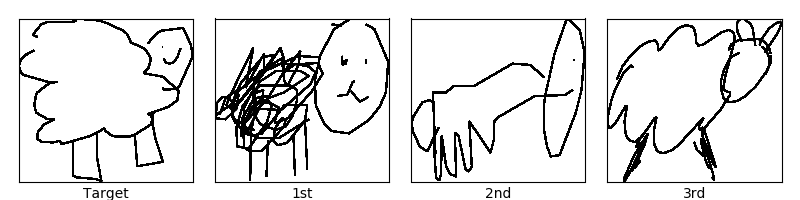
\includegraphics[clip,width=120mm]{sketch_trained_sim_A_0.png}
 		\caption{A}
 		\label{fig:exp1_a}
 	\end{center}
 \end{minipage}

  \begin{minipage}{1\hsize}
  	\begin{center}
  		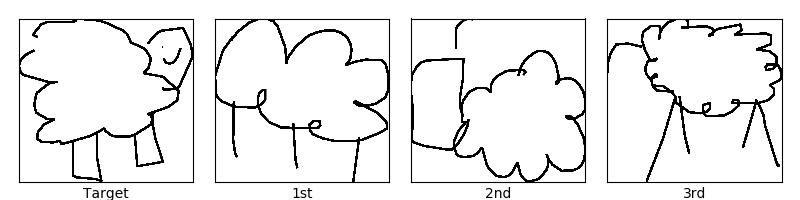
\includegraphics[clip,width=120mm]{sketch_trained_sim_B_0.png}
  		\caption{B}
  		\label{fig:exp1_b}
  	\end{center}
  \end{minipage}

   \begin{minipage}{1\hsize}
   	\begin{center}
   		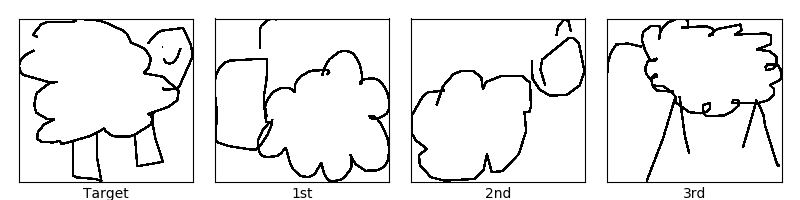
\includegraphics[clip,width=120mm]{sketch_trained_sim_D_0.png}
   		\caption{C}
   		\label{fig:exp1_c}
   	\end{center}
   \end{minipage}
\end{figure*}

類似度の検討

先行研究で用いられていた Structural Similarity (SSIM) は 2 つの画像間での類似指標であり,
一般に画質の劣化を評価するために利用される.
先行研究はこの類似度指標について議論されており,
変換前の生のスケッチについて,「描き順」と画像化した「最終状態」の 2 つを考慮した複雑な指標となっていた.

あまりに複雑なのでまずは,変換後の潜在変数についてコサイン類似度を使ってスケッチを比較した.

\subsection{実験設定}

\begin{table}[tb]
  \begin{center}
    \caption{実験1の設定}
    \begin{tabular}{|c|c|} \hline
       & name \\ \hline
      step & 150,000 \\ \hline
      class & 345 \\ \hline
      latent & (128, ) \\ \hline
      learning rate & 0.0000 \\ \hline
      learning rate & 0.0000 \\ \hline
      learning rate & 0.0000 \\ \hline
      learning rate & 0.0000 \\ \hline
      learning rate & 0.0000 \\ \hline
    \end{tabular}
    \label{tab:setting1}
  \end{center}
\end{table}

ここにテキストを入力してください.ここにテキストを入力してください.ここにテキストを入力してください.ここにテキストを入力してください.ここにテキストを入力してください.ここにテキストを入力してください.

\subsection{結果}
% A[(7, 0.9862899), (6, 0.89415294), (2, 0.7782751), (1, 0.57062423), (8, 0.4869256), (0, 0.0013451368), (3, -0.21240741), (9, -0.21476299), (5, -0.5499855), (4, -0.9028328)]
% B[(8, -116.04807692307692), (1, -116.8173076923077), (5, -118.45192307692308), (3, -120.98076923076923), (9, -121.09615384615384), (2, -121.10576923076923), (4, -122.03846153846153), (0, -130.45192307692307), (6, -131.46153846153845), (7, -131.46153846153845)]
% = [(8, 0.3675329896053509), (1, 0.3032792943562569), (5, 0.15298536646415564), (3, -0.09760859402959103), (9, -0.10896271676452136), (2, -0.10990703386698913), (4, -0.1997384988151555), (0, -0.7225552339045035), (6, -0.7535157530723093), (7, -0.7535157530723093)]

% C[(8, 1.0934066387256818), (5, 0.9155709468131241), (1, 0.2629781539584698), (6, 0.228598204332781), (7, 0.17851659365315453), (2, -0.05635251758133125), (3, -0.9260878840381359), (9, -1.0704136511746165), (4, -1.1764581166587835), (0, -1.580862833925866)]
% D[(1, 1.511369831256345), (4, 1.341358246262741), (5, 0.5409496028127758), (8, -0.017384995408811332), (9, -0.06231150135711422), (3, -0.1333689828363287), (2, -0.16729802033620456), (6, -0.6606084867923497), (0, -0.831266857121777), (7, -0.8643148704974889)]


図 ~ に実験 1 の結果を示す.
% y=\frac{\frac{\left(120-x\right)}{10}}{\left(1+\frac{\left(120-x\right)}{10}^{2}\right)^{0.5}}

データセット内に含まれる 2 つのイラストを取り出し,エンコードした潜在変数 $z$ (= 128 次元)をコサイン類似度で評価した.結果を図 ~ に示す.

まずコサイン類似度自体を評価すると,同一のイラストでは 1 になり機能している可能性は高いが,その他の例ではかなり絶対値が小さくなった.
% まだ詳しくはわかっていないが次元の呪いが関係しているかもしれない.
先行研究は 1 ストロークごとに評価していたと認識しているので,複雑な形状だとそもそも難しいということも考えられる.

\section{実験2: スケッチデータの変換}
スケッチを正順,逆順,シャッフル,分割など,描き順を変換できるようにした.

(変換後の順序は別資料のgifを参考にする)

ここにテキストを入力してください.ここにテキストを入力してください.ここにテキストを入力してください.ここにテキストを入力してください.ここにテキストを入力してください.ここにテキストを入力してください.

分割方法の説明.

データセットの説明.

\subsection{結果}

今回は,逆順とシャッフルについてそれぞれ正順と再構築した結果を比較した.
逆順はほとんど復元できているものが少なく,直線で終わる結果が多かった.
おそらくスケッチの最後は目やしっぽなど,小さな特徴を描き足していく段階で,
内部のベクトルが飛び飛びになるものが RNN にとって難しいくデータも少ないため,
上手くいかなかったと考えられる.
最終的な状態は同じでもやはり内部の潜在変数は,大きく異るようである.

シャッフルでは場合によって,
オリジナルと比較すると復元できていると言えるものもあった.
元データは人間が書いたものなので,
逆順よりは人間に近い変換になりやすかったのだと考えられる.

\begin{figure*}[tb]
 \begin{minipage}{0.5\hsize}
 	\begin{center}
 		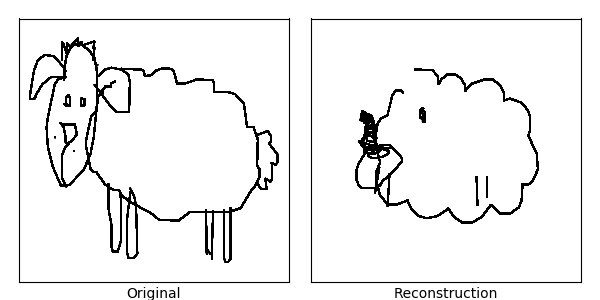
\includegraphics[clip,width=75mm]{sketch_tra_reverse_org_0.png}
 		\caption{逆順スケッチ:オリジナル}
 		\label{fig:short}
 	\end{center}
 \end{minipage}
 \begin{minipage}{0.5\hsize}
 	\begin{center}
    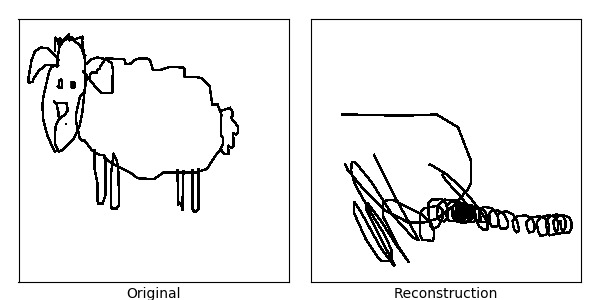
\includegraphics[clip,width=75mm]{sketch_tra_reverse_rvr_0.png}
    \caption{逆順スケッチ:変換後}
    \label{fig:param}
 	\end{center}
 \end{minipage}
\end{figure*}

\begin{figure*}[tb]
 \begin{minipage}{0.5\hsize}
 	\begin{center}
 		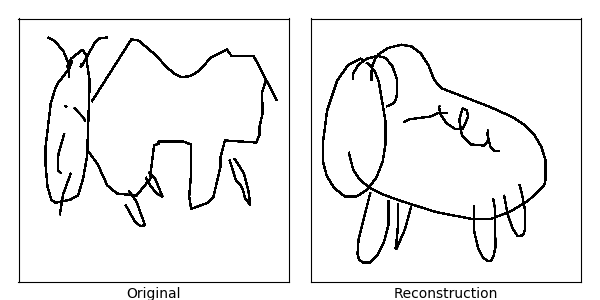
\includegraphics[clip,width=75mm]{sketch_tra_shuffle_org_0.png}
 		\caption{シャッフルスケッチ:オリジナル}
 		\label{fig:short}
 	\end{center}
 \end{minipage}
 \begin{minipage}{0.5\hsize}
 	\begin{center}
    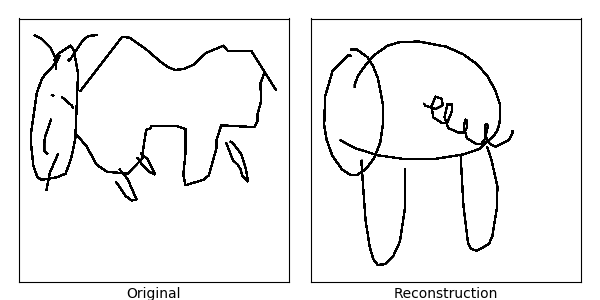
\includegraphics[clip,width=75mm]{sketch_tra_shuffle_rvr_0.png}
    \caption{シャッフルスケッチ:変換後}
    \label{fig:param}
 	\end{center}
 \end{minipage}
\end{figure*}


\section{まとめと今後の課題}
書き順を含むスケッチデータに対して~実験をし,類似度指標の考察をした.

絵描き歌用のデータセットを整備すること.

分割したクラスに対して言語モデルを通して,絵描き歌の歌詞を生成することが課題としてあげられる.

ここにテキストを入力してください.ここにテキストを入力してください.ここにテキストを入力してください.ここにテキストを入力してください.ここにテキストを入力してください.ここにテキストを入力してください.ここにテキストを入力してください.ここにテキストを入力してください.

% 参考文献リスト
\bibliographystyle{unsrt}
\bibliography{ref}
\end{document}
